\documentclass{article}

% if you need to pass options to natbib, use, e.g.:
%     \PassOptionsToPackage{numbers, compress}{natbib}
% before loading neurips_2020

% ready for submission
% \usepackage{neurips_2020}

% to compile a preprint version, e.g., for submission to arXiv, add add the
% [preprint] option:
    % \usepackage[preprint,nonatbib]{neurips_2020}

% to compile a camera-ready version, add the [final] option, e.g.:
    \usepackage[final]{neurips_2020}

% to avoid loading the natbib package, add option nonatbib:
    %  \usepackage[nonatbib]{neurips_2020}

\usepackage{graphics}
\usepackage{textcomp}
\usepackage{graphicx}
\usepackage{wrapfig}
\usepackage{amsfonts}
\usepackage{algorithm,algorithmicx}
\usepackage{algpseudocode}
\usepackage{microtype}      % microtypography
\usepackage{pdfpages}
\usepackage{amsmath}
\usepackage{amssymb}
\usepackage{float}
\usepackage{amsthm}
\usepackage{multicol}
\usepackage[toc,page]{appendix}
\usepackage{balance} % for balancing columns on the final page
\usepackage{caption} 
\usepackage{hyperref}
\hypersetup{
    colorlinks=true,
    linkcolor=blue,
    urlcolor=blue,
    citecolor=blue
}

\newtheorem{innercustomgeneric}{\customgenericname}
\providecommand{\customgenericname}{}
\newcommand{\newcustomtheorem}[2]{%
  \newenvironment{#1}[1]
  {%
   \renewcommand\customgenericname{#2}%
   \renewcommand\theinnercustomgeneric{##1}%
   \innercustomgeneric
  }
  {\endinnercustomgeneric}
}

\newcustomtheorem{customthm}{Theorem}
\newcustomtheorem{customlemma}{Lemma}

\title{Energy-based Surprise Minimization for Multi-Agent Value Factorization}

% The \author macro works with any number of authors. There are two commands
% used to separate the names and addresses of multiple authors: \And and \AND.
%
% Using \And between authors leaves it to LaTeX to determine where to break the
% lines. Using \AND forces a line break at that point. So, if LaTeX puts 3 of 4
% authors names on the first line, and the last on the second line, try using
% \AND instead of \And before the third author name.

\author{
  Karush Suri$^{1}$, Xiao Qi Shi$^{2}$, Konstantinos Plataniotis$^{1}$ and Yuri Lawryshyn$^{1}$\\
   $^{1}$University of Toronto $^{2}$RBC Capital Markets\\
  \texttt{karush.suri@mail.utoronto.ca}
}


\begin{document}

\maketitle

\begin{abstract}
 Multi-Agent Reinforcement Learning (MARL) has demonstrated significant success in training decentralised policies in a centralised manner by making use of value factorization methods. However, addressing surprise across spurious states and approximation bias remain open problems for multi-agent settings.  We introduce the Energy-based MIXer (EMIX), an algorithm which minimizes surprise utilizing the energy across agents. Our contributions are threefold; (1) EMIX introduces a novel surprise minimization technique across multiple agents in the case of multi-agent partially-observable settings. (2) EMIX highlights the first practical use of energy functions in MARL (to our knowledge) with theoretical guarantees and experiment validations of the energy operator. Lastly, (3) EMIX presents a novel technique for addressing overestimation bias across agents in MARL. When evaluated on a range of challenging StarCraft II micromanagement scenarios, EMIX demonstrates consistent state-of-the-art performance for multi-agent surprise minimization. Moreover, our ablation study highlights the necessity of the energy-based scheme and the need for elimination of overestimation bias in MARL. Our implementation of EMIX, videos of agents and blog are available in the supplementary material. 
\end{abstract}

\begin{multicols}{2}
\section{Introduction}
Reinforcement Learning (RL) has seen tremendous growth in applications such as arcade games \cite{atari}, board games \cite{go, shogi}, robot control tasks \cite{ddpg, ppo} and lately, real-time games \cite{SC2}. The rise of RL has led to an increasing interest in the study of multi-agent systems \cite{maddpg, alphastar}, commonly known as Multi-Agent Reinforcement Learning (MARL). In the case of partially observable settings, MARL enables the learning of policies with centralised training and decentralised control \cite{dec}. This has proven to be useful for exploiting value-based methods which are often found to be sample-inefficient \cite{iql,coma}. Value Factorization \cite{vdn,qmix} is a common technique which enables the joint value function to be represented as a combination of individual value functions. In the case of Value Decomposition Network (VDN) \cite{vdn}, a linear additive factorization is carried out whereas QMIX \cite{qmix} generalizes the factorization to a non-linear combination, hence improving the expressive power of centralised action-value functions. Furthermore, monotonicity constraints in QMIX enable scalability in the number of agents. On the other hand, factorization across multiple value functions leads to the aggregation of approximation biases \cite{doubleqlearning, deepdoubleqlearning} originating from overoptimistic estimations in action values \cite{td3,maxmin} which remain an open problem in the case of multi-agent settings. Moreover, value factorization methods are conditioned on states and do not account for spurious changes in partially-observed observations, commonly referred to as surprise \cite{surprise}. 

Surprise minimization \cite{smirl} is a recent phenomenon observed in the case of single-agent RL methods which deals with environments consisting of spurious states. In the case of model-based RL \cite{mbrl}, surprise minimization is used as an effective planning tool in the agent's model \cite{smirl} whereas in the case of model-free RL, surprise minimization is witnessed as an intrinsic motivation \cite{surprise,surpmodeling} or generalization problem \cite{gen}. On the other hand, MARL does not account for surprise across agents as a result of which agents remain unaware of drastic changes in the environment \cite{role}. Thus, surprise minimization in the case of multi-agent settings requires attention from a critical standpoint.

We introduce the Energy-based MIXer (EMIX), an algorithm based on QMIX which minimizes surprise utilizing the energy across agents. Our contributions are threefold; (1) EMIX introduces a novel surprise minimization technique across multiple agents in the case of multi-agent partially-observable settings. (2) EMIX highlights the first practical use of energy functions in MARL (to our knowledge) with theoretical guarantees and experiment validations of the energy operator. Lastly, (3) EMIX presents a novel technique for addressing overestimation bias across agents in MARL which, unlike previous single-agent methods \cite{maxmin}, do not rely on a computationally-expensive family of action value functions. When evaluated on a range of challenging StarCraft II scenarios \cite{smac}, EMIX demonstrates state-of-the-art performance for multi-agent surprise minimization by significantly improving the consistent performance of QMIX. Moroever, our ablation study highlights the necessity of our energy-based scheme and the need for elimination of overestimation bias in MARL.

% EMIX makes use of a surprise value function which factorizes states, action values and deviations across partial agent observations into a single surprise value utilizing an energy operator. The surprise value obtained is then used in conjunction with the joint action value function to yield the EMIX objective. EMIX additionally addresses estimation bias in the joint action value function by making use of dual target functions which, unlike previous single-agent methods \cite{maxmin}, do not rely on a computationally-expensive family of action value functions.

%%%%%%%%%%%%%%%%%%%%%%%%%%%%%%%%%%%%%%%%%%%%%%%%%%%%%%%%%%%%%%%%%%%%%%%%

\section{The Value Factorization Problem}
\subsection{Preliminaries}
We review the cooperative MARL setup. The problem is modeled as a Partially Observable Markov Decision Process (POMDP) \cite{rl} defined by the tuple $(\mathcal{S},\mathcal{A},r,N,P,Z,O,\gamma)$ where the state space $\mathcal{S}$ and action space $\mathcal{A}$ are discrete, $r: \mathcal{S} \times \mathcal{A} \rightarrow [r_{min},r_{max}]$ presents the reward observed by agents $a \in N$ where $N$ is the set of all agents, $P: \mathcal{S} \times \mathcal{S} \times \mathcal{A} \rightarrow [0,\infty)$ presents the unknown transition model consisting of the transition probability to the next state $s\textquotesingle \in \mathcal{S}$ given the current state $s \in \mathcal{S}$ and joint action $u \in \mathcal{A}$ at time step $t$ and $\gamma$ is the discount factor. We consider a partially observable setting in which each agent $n$ draws individual observations $z \in Z$ according to the observation function $O(s,u): \mathcal{S} \times \mathcal{A} \rightarrow Z$. We consider a joint policy $\pi_{\theta}({u|s})$ as a function of model parameters $\theta$. Standard RL defines the agent's objective to maximize the expected discounted reward $\mathbb{E}_{\pi_{\theta}}[\sum_{t=0}^{T}\gamma^{t}r(s_{t},u_{t})]$ as a function of the parameters $\theta$. The action-value function for an agent is represented as $Q(u,s;\theta) = \mathbb{E}_{\pi_{\theta}}[\sum_{t=1}^{T}\gamma^{t}r(s,u)|s=s_{t},u=u_{t}]$ which is the expected sum of payoffs obtained in state $s$ upon performing action $u$ by following the policy $\pi_{\theta}$. We denote the optimal policy $\pi_{\theta}^{*}$ such that $Q(u,s;\theta^{*}) \geq Q(u,s;\theta) \forall s \in S, u \in A$. In the case of multiple agents, the joint optimal policy can be expressed as the Nash Equilibrium \cite{nash} of the Stochastic Markov Game as $\pi^{*} = (\pi^{1,*},\pi^{2,*}, ...\pi^{N,*})$ such that $Q(u^{a},s;\theta^{*}) \geq Q(u^{a},s;\theta) \forall s \in S, u \in A, a \in N$. Q-Learning is an off-policy, model-free algorithm suitable for continuous and episodic tasks. The algorithm uses semi-gradient descent to minimize the Temporal Difference (TD) error: $\mathbb{L(\theta)} = \underset{b \sim R}{\mathbb{E}}[(y - Q(u,s;\theta))^{2}]$ where $y = r + \gamma \underset{u^{\textquotesingle}\in A}{\max} Q(u^{\textquotesingle},s^{\textquotesingle};\theta^{-})$ is the TD target consisting of $\theta^{-}$ as the target parameters and $b$ is the batch sampled from memory $R$.

\subsection{Surprise Minimization}
Despite the recent success of value-based methods \cite{a3c,rainbow} RL agents suffer from spurious state spaces and encounter sudden changes in trajectories. These anomalous transitions between consecutive states are termed as surprise \cite{surprise}. Quantitatively, surprise can be inferred as a measure of deviation \cite{smirl,gen} among states encountered by the agent during its interaction with the environment. While exploring \cite{curiosity,exploration} the environment, agents tend to have higher deviation among states which is gradually reduced by gaining a significant understanding of state-action transitions. Agents can then start selecting optimal actions which is essential for maximizing reward. These actions often lead the agent to spurious experiences which the agent may not have encountered. In the case of model-based RL, agents can leverage spurious experiences \cite{smirl} and plan effectively for future steps. On the other hand, in the case of model-free RL, surprise results in sample-inefficient learning \cite{surprise}. This can be tackled by making use of rigorous exploration strategies \cite{effectiveexp,statemarginal}. However, such techniques do not necessarily scale to high-dimensional tasks and often require extrinsic feature engineering \cite{hdqn} and meta models \cite{metaexp}. A suitable way to tackle high-dimensional dynamics is by utilizing surprise as a penalty on the reward \cite{gen}. This leads to improved generalization. However, such solutions do not show evidence for multiple agents consisting of individual partial observations \cite{marlsurp}. 

\subsection{Overestimation Bias}
Recent advances \cite{td3} in value-based methods have addressed overestimation bias (also known as approximation error) which stems from the value estimates approximated by the function approximator. Such methods make use of dual target functions \cite{duel} which improve stability in the Bellman updates. This has led to a significant improvement in single-agent off-policy RL methods \cite{sac}. However, MARL value-based methods continue to suffer from overestimation bias \cite{marlover,iqn}. \autoref{fig:tderror} highlights the overestimation bias originating from the overoptimistic estimations of the target value estimator. Plots present the variation of absolute TD error during learning for state-of-the-art MARL methods, namely Independent Q-Learning \cite{iql}, Counterfactual Multi-Agent Policy Gradients (COMA) \cite{coma}, VDN \cite{vdn} and QMIX \cite{qmix}. Significant rise in error values of value factorization methods such as QMIX and VDN presents the aggregation of errors from individual $Q$-value functions. Thus, overestimation bias in MARL value factorization requires attention from a critical standpoint.

\begin{wrapfigure}{r}{6cm}
    \centering
    
\includegraphics[height=2.5cm,width=6cm]{tderror.png}
    \caption{Absolute TD error for state-of-the-art MARL methods in StarCraft II micromanagement scenarios. Rise in error values depict the overoptimistic approximations estimated by the target value estimator.}
    \label{fig:tderror}
\end{wrapfigure}


Various MARL methods \cite{twinmix} make use of a dual architecture approach which increases the stability in value factorization. However, these methods are only applicable to small set of micromanagement tasks and do not generalize to scenarios consisting of a larger number of opponents and environments with different dynamics. Another suitable approach observed in literature is the usage of weighted bellman updates in double Q-learning \cite{weightdouble}. The Weighted Double Deep $Q$-Network (WDDQN) provides stability and sample efficiency for fully-observable MDPs. In the case of cooperative POMDPS, Weighted-QMIX (WQMIX) \cite{wqmix} yields a more sophisticated weighting scheme which aids in the retrieval of optimal policy \cite{challenges}. Although suitable for value factorization in challenging micromanagement tasks, the method needs to be carefully hand-engineered and, in the case of multiple weighting schemes, does not include a basis for selection. A more practical approach in the case of single-agent methods is the use of a family of $Q$-functions \cite{maxmin} wherein each estimator is optimized individually. Such a framework provides a generalized method for training agents with greedy policies and minimum approximation error. Although successful in single-agent settings, generalized Q-function methods do not scale well in the number of agents \cite{challenges} since each agent requires a family of $Q$-functions which needs to be updated concurrently. Thus, addressing overestimation bias from value factorization in cooperative multi-agent frameworks requires a scalable and sample-efficient perspective.  

\subsection{Energy-based Models}
Energy-Based Models (EBMs) \cite{ebm,ebmdoc} have been successfully applied in the field of machine learning \cite{energy} and probabilistic inference \cite{david}. A typical EBM $\mathcal{E}$ formulates the equilibrium probabilities \cite{rlhinton} $P(v,h) = \frac{\exp{(-\mathcal{E}(v,h))}}{\sum_{\hat{v},\hat{h}}[\exp{(-\mathcal{E}(\hat{v},\hat{h}))}]}$ via a Boltzmann distribution \cite{boltzmann} where $v$ and $h$ are the values of the visible and hidden variables and $\hat{v}$ and $\hat{h}$ are all the possible configurations of the visible and hidden variables respectively. The probability distribution over all the visible variables can be obtained by summing over all possible configurations of the hidden variables. This is mathematically expressed in \autoref{eq:1}.
\begin{gather}
    P(v) = \frac{\sum_{h}[\exp{(-\mathcal{E}(v,h))}]}{\sum_{\hat{v},\hat{h}}[\exp{(-\mathcal{E}(\hat{v},\hat{h}))}]} \label{eq:1}    
\end{gather}
Here, $\mathcal{E}(v,h)$ is called the equilibrium free energy which is the minimum of the variational free energy and $\sum_{\hat{v},\hat{h}}[\exp{(-\mathcal{E}(\hat{v},\hat{h}))}]$ is the partition function. EBMs have been successfully implemented in single-agent RL methods \cite{pgq,sql}. These typically make use of Boltzmann distributions to approximate policies \cite{boltzmann}. Such a formulation results in the minimization of free energy within the agent. While policy approximation depicts promise in the case of unknown dynamics, inference methods \cite{inference} play a key role in optimizing goal-oriented behavior. A second type of usage of EBMs follows the maximization of entropy \cite{ziebartinverse}. The maximum entropy framework \cite{sac} highlighted in Soft Q-Learning (SQL) \cite{sql} allows the agent to obey a policy which maximizes its reward and entropy concurrently. Maximization of agent's entropy results in diverse and adaptive behaviors \cite{ziebartphd} which may be difficult to accomplish using standard exploration techniques \cite{curiosity,exploration}. Moreover, the maximum entropy framework is equivalent to approximate inference in the case of policy gradient methods \cite{equivalence}. Such a connection between likelihood ratio gradient techniques and energy-based formulations leads to diverse and robust policies \cite{haarnoja} and their hierarchical extensions \cite{hierarchical} which preserve the lower levels of hierarchies.

In the case of MARL, EBMs have witnessed limited applicability as a result of the increasing number of agents and complexity within each agent \cite{overview}. While the probabilistic framework is readily transferable to opponent-aware multi-agent systems \cite{probabilistic}, cooperative settings consisting of coordination between agents require a firm formulation of energy which is scalable in the number of agents \cite{twoplayer} and accounts for environments consisting of spurious states \cite{marlsql}. 
%%%%%%%%%%%%%%%%%%%%%%%%%%%%%%%%%%%%%%%%%%%%%%%%%%%%%%%%%%%%%%%%%%%%%%%%

\section{Energy-based Surprise Minimization}
In this section we introduce the novel surprise minimizing EMIX agent. The motivation behind EMIX stems from spurious states and overestimation bias among agents in the case of partially-observed settings. EMIX aims to address these challenges by making use of an energy-based surprise value function in conjunction with dual target function approximators. 

\subsection{The Surprise Minimization Objective}
Firstly, we formulate the energy-based objective consisting of surprise as a function of states $s$, joint actions $u$ and deviation $\sigma$ within states for each agent $a$. We call this function as the surprise value function $V_{surp}^{a}(s,u,\sigma)$ which serves as a mapping from agent and environment dynamics to surprise. We then define an energy operator presented in \autoref{eq:2} which sums the free energy across all agents. 
\begin{gather}
    \mathcal{T}V^{a}_{surp}(s,u,\sigma) = \log \sum_{a=1}^{N} \exp{(V^{a}_{surp}(s,u,\sigma))} \label{eq:2}
\end{gather}
We make use of the Mellowmax operator \cite{mellowmax} as our energy operator. The energy operator is similar to the SQL energy formulation \cite{sql} where the energy across different actions is evaluated. In our case, inference is carried out across all agents with actions as prior variables. However, in the special case of using an EBM as a $Q$-function, the EMIX objective reduces to the SQL objective (details in the supplementary material). 

Our choice of the energy operator is based on its unique mathematical properties which result in better convergence. Of these properties, the most useful result is that the energy operator forms a contraction on the surprise value function indicating a guaranteed minimization of surprise within agents. This is formally stated in Theorem \autoref{one}. Proof of Theorem \autoref{one} can be found in the supplementary material. % refer here
\begin{customthm}{1}\label{one}
Given a surprise value function $V^{a}_{surp}(s,u,\sigma) \forall a \in N$, the energy operator $\mathcal{T}V^{a}_{surp}(s,u,\sigma)=\log \sum_{a=1}^{N} \exp{(V^{a}_{surp}(s,u,\sigma))}$ forms a contraction on $V^{a}_{surp}(s,u,\sigma)$. 
\end{customthm}
The energy-based surprise minimization objective can then be formulated by simply adding the approximated energy-based surprise to the initial Bellman objective as expressed below.
\begin{equation}
    \begin{aligned}
    L(\theta) = \underset{b \sim R}{\mathbb{E}}[\frac{1}{2}(y - (Q(u,s;\theta) + \beta \log \sum_{a=1}^{N} \exp{(V^{a}_{surp}(s,u,\sigma))}))^{2}] \nonumber
    \end{aligned}
\end{equation}
where $y = r + \gamma \underset{u^{'}}{\max}Q(u^{'},s^{'};\theta^{-}) + \beta \log \sum_{a=1}^{N} \exp{(V^{a}_{surp}(s^{'},u^{'},\sigma^{'}))}$. This yields the following,
\begin{gather*}
     = \underset{b \sim R}{\mathbb{E}}[\frac{1}{2}(r + \gamma \underset{u^{'}}{\max}Q(u^{'},s^{'};\theta^{-}) + \beta \log \frac{\sum_{a=1}^{N} \exp{(V^{a}_{surp}(s^{'},u^{'},\sigma^{'}))}}{\sum_{a=1}^{N} \exp{(V^{a}_{surp}(s,u,\sigma))}} - Q(u,s;\theta))^{2}]
\end{gather*}
\begin{gather}
    L(\theta) = \underset{b \sim R}{\mathbb{E}}[\frac{1}{2}(r + \gamma \underset{u^{'}}{\max}Q(u^{'},s^{'};\theta^{-}) + \beta E - Q(u,s;\theta))^{2}] \label{eq:3}
\end{gather}
Here, $E$ is defined as the surprise ratio with $\beta$ as a temperature parameter and $\sigma^{'}$ as the deviation among next states in the batch. The surprise value function is approximated by a universal function approximator (in our case a neural network) with its parameters as $\phi$. $V_{a}(s^{'},u^{'},\sigma^{'})$ is expressed as the negative free energy and $\sum_{a=1}^{N} \exp{(V_{a}(s,u,\sigma))}$ the partition function. Alternatively, $V_{a}(s,u,\sigma)$ can be formulated as the negative free energy with $\sum_{a=1}^{N} \exp{(V_{a}(s^{'},u^{'},\sigma^{'}))}$ as the partition function. The objective incorporates the minimization of surprise across all agents as minimizing the energy in spurious states. Such a formulation of surprise acts as intrinsic motivation and at the same time provides robustness to multi-agent behavior. Furthermore, the energy formulation in the form of energy ratio $E$ is a suitable one as it guarantees convergence to minimum surprise at optimal policy $\pi^{*}$. This is formally expressed in Theorem \autoref{two} with its corresponding proof in the supplementary material.
\begin{customthm}{2}\label{two}
Upon agent's convergence to an optimal policy $\pi^{*}$, total energy of $\pi^{*}$, expressed by $E^{*}$ will reach a thermal equilibrium consisting of minimum surprise among consecutive states $s$ and $s^{'}$.
\end{customthm}
The objective can be modified to tackle approximation error in the target $Q$-values. We introduce a total of $m$ target approximators making $\{Q_{1}(u^{'},s^{'};\theta^{-}),Q_{2}(u^{'},s^{'};\theta^{-})...,Q_{m}(u^{'},s^{'};\theta^{-})\}$ as the set of target approximators. However, unlike generalized $Q$-learning \cite{maxmin}, we do not instantiate another $Q$-function but simply keep a copy of $\theta$ and select the target estimates with minimum values during optimization. This allows the objective to address overestimation bias in a scalable manner without using multiple $Q$-functions. The final EMIX objective is mathematically expressed in \autoref{eq:4}.
\begin{gather}
    L(\theta) = \underset{b \sim R}{\mathbb{E}}[\frac{1}{2}(r + \gamma \underset{u^{'}}{\max}\underset{i}{\min}Q_{i}(u^{'},s^{'};\theta^{-}) + \beta E - Q(u,s;\theta))^{2}] \label{eq:4}
\end{gather}
Here, $i$ depicts each of the $m$ target estimators with $\underset{i}{\min}Q_{i}(u^{'},s^{'};\theta^{-})$ indicating the estimate with minimum error. 

\subsection{Energy-based MIXer (EMIX)}
\begin{algorithm}[H]
\caption{Energy-based MIXer (EMIX)}
\label{alg:algorithm1}
\begin{algorithmic}[1]

  % INITIALIZE EVERYTHING
  \State Initialize $\phi$, $\theta$, $\theta_{1}^{-}...,\theta_{m}^{-}$, agent and hypernetwork parameters.
  \State Initialize learning rate $\alpha$, temperature $\beta$ and replay buffer $\mathcal{R}$.

  % MAIN LOOP
  \For{environment step}
      \State $u \xleftarrow[]{} (u_{1},u_{2}...,u_{N})$
      \State $\mathcal{R} \xleftarrow[]{} \mathcal{R} \cup \{(s,u,r,s^{'})\}$
      \If{$|\mathcal{R}| >$ batch-size}
        \For{random batch}
            \State $Q_{tot}^{\theta} \xleftarrow[]{}$ \textit{Mixer-Network}($Q_{1},Q_{2}...,Q_{N},s$)
            \State $Q_{i}^{\theta^{-}} \xleftarrow[]{}$ \textit{Target-Mixer}$_{i}$($Q_{1},Q_{2}...,Q_{N},s^{'}$),  $\forall i=1,2..,m$
            \State Calculate $\sigma$ and $\sigma^{'}$ using $s$ and $s^{'}$
            \State $V_{surp}^{a}(s,u,\sigma) \xleftarrow[]{}$ \textit{Surprise-Mixer($s,u,\sigma$)}
            \State $V_{surp}^{a}(s^{'},u^{'},\sigma^{'}) \xleftarrow[]{}$ \textit{Target-Surprise-Mixer($s^{'},u^{'},\sigma^{'}$)}
            \State $E \xleftarrow[]{} \log \frac{\sum_{a=1}^{N} \exp{(V^{a}_{surp}(s^{'},u^{'},\sigma^{'}))}}{\sum_{a=1}^{N} \exp{(V^{a}_{surp}(s,u,\sigma))}}$
            \State Calculate $L(\theta)$ using $E$ in \autoref{eq:4}
            \State $\theta \xleftarrow[]{} \theta - \alpha \nabla_{\theta}L(\theta)$
        \EndFor
    \EndIf
    \If{update-interval steps have passed}
        \State $\theta_{i}^{-} \xleftarrow[]{} \theta, \forall i=1,2..,m$
    \EndIf
  \EndFor

\end{algorithmic}
\end{algorithm}

Algorithm \autoref{alg:algorithm1} presents the EMIX algorithm. We initialize surprise value function parameters $\phi$, mixer parameters $\theta$, target parameters $\theta_{i}^{-}$ for $i=1,2...,m$ and lastly the agent and hypernetwork parameters of QMIX. A learning rate $\alpha$, temperature $\beta$ and replay buffer $\mathcal{R}$ are instantiated. During environment interactions, agents in state $s$ perform joint action $u$, observe reward $r$ and transition to next-states $s^{'}$. These experiences are collected in $\mathcal{R}$ as $(s,u,r,s^{'})$ tuples. In order to make the agents explore the environment, an $\epsilon$-greedy schedule is used similar to the original QMIX \cite{qmix} implementation. During the update steps, a random batch of $batch-size$ is sampled from $\mathcal{R}$. The total $Q$-value $Q_{tot}^{\theta}$ is computed by the mixer network with its inputs as the $Q$-values of all the agents conditioned on $s$ via the hypernetworks. Similarly, the target mixers approximate $Q_{i}^{\theta^{-}}$ conditioned on $s^{'}$. In order to evaluate surprise within agents, we compute the standard deviations $\sigma$ and $\sigma^{'}$ across all observations $z$ and $z^{'}$ for each agent using $s$ and $s^{'}$ respectively. The surprise value function called the Surprise-Mixer estimates the surprise $V^{a}_{surp}(s,u,\sigma)$ conditioned on $s$, $u$ and $\sigma$. The same computation is repeated using the Target-Surprise-Mixer for estimating surprise $V^{a}_{surp}(s^{'},u^{'},\sigma^{'})$  within next-states in the batch. Application of the energy operator along the non-singleton agent dimension for $V^{a}_{surp}(s,u,\sigma)$ and $V^{a}_{surp}(s^{'},u^{'},\sigma^{'})$ yields the energy ratio $E$ which is used in \autoref{eq:4} to evaluate $L(\theta)$. We then use batch gradient descent to update parameters of the mixer $\theta$. Target parameters $\theta_{i}^{-}$ are updated every $update-interval$ steps.
\begin{wrapfigure}{r}{6cm}
    \centering
    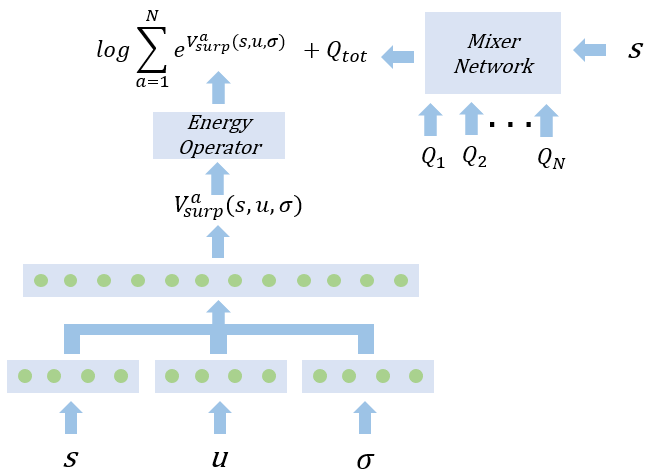
\includegraphics[height=4cm,width=6cm]{emix.PNG}
    \caption{Surprise-Mixer architecture for estimation of the surprise value function.}
    \label{fig:emix}
\end{wrapfigure}
We now take a closer look at the surprise-mixer approximating the surprise value function. In order to condition surprise on states, joint actions and the deviation among states, we construct an expressive architecture motivated by provable exploration in RL \cite{homer}. The original architecture constructs a state abstraction model for a classification setting. It maps the transitions consisting of states $s$, actions $u$ and next-states $s^{'}$ to the conditional probability $p(y|s,a,s^{'})$ depicting whether the transition belongs to the same data distribution $y$ or not. Such models have proven to be efficient in the case of provable exploration \cite{homer} as it allows the agent to learn an exploration policy for every value of abstract state related to the latent space. We borrow from this technique of provable exploration and extend it to the surprise minimization setting.

\autoref{fig:emix} presents the expressive architecture of surprise-mixer network utilized for surprise value function approximation and minimization. In contrast to the original state abstraction model \cite{homer}, the surprise-mixer maps transitions consisting of states $s$, joint actions $u$ and deviations $\sigma$ to a surprise value $V_{surp}^{a}(s,u,\sigma)$ for all agents $a$. Hierarchical layers of the network aid in the extraction of latent space representations followed by the estimation of $V_{surp}^{a}(s,u,\sigma)$. The architecture allows the agent to learn a robust and surprise-agnostic policy for every value of abstract state related to the latent space. Moreover, the latent space accommodates every value of surprise across agents as a result of state deviations induced in the intermediate representations. Surprise value estimates $V_{surp}^{a}(s,u,\sigma)$ are evaluated by the energy operator with the resulting expression becoming a part of the Bellman objective in \autoref{eq:4} comprising of the total $Q$-values $Q_{tot}$ estimated by the mixer network. 

%%%%%%%%%%%%%%%%%%%%%%%%%%%%%%%%%%%%%%%%%%%%%%%%%%%%%%%%%%%%%%%%%%%%%%%%

\section{Experiments}
Our experiments aim to evaluate the performance, consistency, sample-efficiency and effectiveness of the various components of our method. Specifically, we aim to answer the following questions- (1) How does our method compare to current state-of-the-art MARL methods in terms of performance, consistency and sample efficiency?, (2) How much does each component of the method contribute to its performance? and (3) Does the algorithm validate the theoretical claims corresponding to its components?
\subsection{Energy-based Surprise Minimization}
\begin{table*}[ht]
\resizebox{\textwidth}{!}{
\centering
 \begin{tabular}{c c c c c c c} 
 \hline
 Scenarios & EMIX & SMiRL-QMIX & QMIX & VDN & COMA & IQL \\ [0.5ex] 
 \hline
 2s\textunderscore vs\textunderscore 1sc & 90.33 $\pm$ 0.72 & 88.41 $\pm$ 1.31 & 89.19 $\pm$ 3.23 & 91.42 $\pm$ 1.23 & \textbf{96.90 $\pm$ 0.54} & 86.07 $\pm$ 0.98\\ 
 2s3z & \textbf{95.40$\pm$0.45} & 94.93$\pm$0.32 & 95.30$\pm$1.28 & 92.03$\pm$2.08 & 43.33$\pm$2.70 & 55.74$\pm$6.84\\ 
 3m & \textbf{94.90$\pm$0.39} & 93.94$\pm$0.22 & 93.43$\pm$0.20 & 94.58$\pm$0.58 & 84.75$\pm$7.93 & 94.79$\pm$0.50\\ 
 3s\textunderscore vs\textunderscore 3z & \textbf{99.58$\pm$0.07} & 97.63$\pm$1.08 & 99.43$\pm$0.20 & 97.90$\pm$0.58 & 0.21$\pm$0.54 & 92.32$\pm$2.83\\ 
 3s\textunderscore vs\textunderscore 4z & \textbf{97.22$\pm$0.73} & 0.24$\pm$0.11 & 96.01$\pm$3.93 & 94.29$\pm$2.13 & 0.00$\pm$0.00 & 59.75$\pm$12.22\\ 
 3s\textunderscore vs\textunderscore 5z & 52.91$\pm$11.80 & 0.00$\pm$0.00 & 43.44$\pm$7.09 & \textbf{68.51$\pm$5.60} & 0.00$\pm$0.00 & 18.14$\pm$2.34\\ 
 3s5z & \textbf{88.88$\pm$1.07} & 88.53$\pm$1.03 & 88.49$\pm$2.32 & 63.58$\pm$3.99 & 0.25$\pm$0.11 & 7.05$\pm$3.52\\ 
 8m & \textbf{94.47$\pm$1.38} & 89.96$\pm$1.42 & 94.30$\pm$2.90 & 90.26$\pm$1.12 & 92.82$\pm$0.53 & 83.53$\pm$1.62\\ 
 8m\textunderscore vs\textunderscore 9m & \textbf{71.03$\pm$2.69} & 69.90$\pm$1.94 & 68.28$\pm$2.30 & 58.81$\pm$4.68 & 4.17$\pm$0.58 & 28.48$\pm$22.38\\ 
 10m\textunderscore vs\textunderscore 11m & 75.35$\pm$2.30 & \textbf{77.85$\pm$2.02} & 70.36$\pm$2.87 & 71.81$\pm$6.50 & 4.55$\pm$0.73 & 32.27$\pm$25.68\\ 
 so\textunderscore many\textunderscore baneling & \textbf{95.87$\pm$0.16} & 93.61$\pm$0.94 & 93.35$\pm$0.78 & 92.26$\pm$1.06 & 91.65$\pm$2.26 & 74.97$\pm$6.52\\ 
 5m\textunderscore vs\textunderscore 6m & \textbf{37.07$\pm$2.42} & 33.27$\pm$2.79 & 34.42$\pm$2.63 & 35.63$\pm$3.32 & 0.52$\pm$0.13 & 14.78$\pm$2.72\\ 
 \hline
 \end{tabular}}
 \caption{Comparison of success rate percentages between EMIX and state-of-the-art MARL methods for StarCraft II micromanagement scenarios. Results are averaged over 5 random seeds with each session consisting of 2 million environment interactions. EMIX significantly improves the performance of the QMIX agent on a total of 9 out of 12 scenarios. EMIX demonstrates state-of-the-art performance for surprise minimization on all 12 scenarios in comparison to the SMiRL scheme. In addition, EMIX presents less deviation between its random seeds indicating consistency in collaboration across agents.}
\label{tab:table}
\end{table*}
We assess the performance and sample-efficiency of EMIX on multi-agent StarCraft II micromanagement scenarios \cite{smac} as these consist of a larger number of agents with different action spaces which motivates a greater deal of coordination. Additionally, micromanagement scenarios in StarCraft II consist of multiple opponents which introduce a greater degree of surprise within consecutive states. We compare our method to current state-of-the-art methods, namely QMIX \cite{qmix}, VDN \cite{vdn}, COMA \cite{coma} and IQL \cite{iql}. In order to compare our surprise-based scheme against pre-existing surprise minimization mechanisms, we compare EMIX additionally to a model-free implementation of SMiRL \cite{smirl} in QMIX. All methods were implemented using the PyMARL framework \cite{smac}. The SMiRL component was additionally incorporated as per the update rule provided in \cite{gen}. We use the generalized version of SMiRL as it demonstrates reduced variance across batches. We term this implementation as SMiRL-QMIX for our comparisons. Details related to the implementation of EMIX are presented in the supplementary material.

\autoref{tab:table} presents the comparison of success rate percentages between EMIX and state-of-the-art MARL algorithms on the StarCraft II micromanagement scenarios. Along with the success rates, we also measure the deviation of performance across the 5 random seeds considered during experiments. (complete results in supplementary material). We evaluate the performance of agents on a total of 12 scenarios. Corresponding to each scenario, algorithms demonstrating higher success rate values in comparison to other methods have their entries highlighted. Out of the 12 scenarios considered, EMIX presents higher success rates on 9 of these scenarios depicting the suitability of the proposed approach. EMIX presents significant performance gains in cases of \textit{so\textunderscore many\textunderscore baneling} and \textit{5m\textunderscore vs \textunderscore 6m} which consist of a large number of opponents and a greater difficulty level respectively. When compared to QMIX, EMIX depicts improved success rates on all of the 12 scenarios. For instance, in scenarios such as \textit{3s\textunderscore vs\textunderscore 5z}, \textit{8m\textunderscore vs\textunderscore 9m} and \textit{5m\textunderscore vs\textunderscore 6m} QMIX presents sub-optimal performance whereas EMIX utilizes a comparatively improved joint policy and yields better convergence in a sample-efficient manner. Moreover, on comparing EMIX with SMiRL-QMIX, we note that EMIX demonstrates a higher average success rate. This highlights the suitability of the energy-based scheme in the case of a larger number of agents and complex environment dynamics for surprise minimization.

\subsection{Ablation Study}
% \begin{figure*}[ht]
%     \centering
%     \includegraphics[height=2cm,width=14cm]{ablations.png}
%     \includegraphics[height=2cm,width=14cm]{surprise.png}
%     \caption{Ablations on six different scenarios for each of EMIX's component ablations (top) and variation of surprise minimization (bottom) with temperature $\beta$. When compared to QMIX, EMIX and TwinQMIX depict improved performance and sample efficiency. This is achieved by making use of a suitable value of temperature parameter ($\beta=0.01$) which controls the stability in surprise minimization by utilizing $E$ as intrinsic motivation.}
%     \label{fig:ablations}
% \end{figure*}
We now present the ablation study for the various components of EMIX. Our experiments aim to determine the effectiveness of the energy-based surprise minimization method and the multiple target $Q$-function scheme. Additionally, we also aim to determine the extent up to which our proposed framework is viable in the standard QMIX objective.

\textbf{EMIX Objective}: To weigh the effectiveness of the multiple target $Q$-function scheme we remove the energy-based surprise minimization from EMIX and replace it with the prior QMIX objective. For simplicity, we make use of two target $Q$-functions. We call this implementation of QMIX combined with the dual target function scheme as \textit{TwinQMIX}. We can now add the energy-based surprise minimization scheme in the TwinQMIX objective to retrieve the EMIX objective. Thus, we can compare between QMIX, TwinQMIX and EMIX to assess the contributions of each of the proposed methods. \autoref{fig:ablations} (top) presents the comparison of average success rates for QMIX, TwinQMIX and EMIX on six different scenarios. Agents were evaluated for a total of 2 million timesteps with the lines in the plot indicating average success rates and the shaded area as the deviation across 5 random seeds. In comparison to QMIX, TwinQMIX adds stability to the original objective by reducing the overoptimistic estimates in the initial QMIX objective. On comparing TwinQMIX to EMIX we note that the energy-based surprise minimization scheme provides significant performance improvement in the modified QMIX objective. This is demonstrated in the \textit{5m\textunderscore vs\textunderscore 6m} scenario wherein the EMIX implementation improves the performance of TwinQMIX in comparison to QMIX by utilizing a surprise-robust policy. In the case of \textit{so\textunderscore many \textunderscore baneling} scenario which consists of a large number of opponents (27 banelings), EMIX tackles surprise effectively by preventing a significant drop in performance which is observed in cases of QMIX and TwinQMIX.

\textbf{Temperature Parameter}: The importance of $\beta$ can be validated by assessing its usage in surprise minimization. However, it is difficult to evaluate surprise minimization directly as surprise value function estimates $V_{surp}^{a}(s,u,\sigma)$ vary from state-to-state across different agents and thus, they present high variance during agent's learning. This, in turn poses hindrance to gain an intuitive understanding of the surprise distribution. We instead observe the variation of $E$ as it is a collection of surprise-based sample estimates across the batch. Additionally, $E$ consists of prior samples $V_{surp}^{a}(s,u,\sigma)$ for $V_{surp}^{a}(s^{'},u^{'},\sigma^{'})$ which makes inference across different agents tractable. \autoref{fig:ablations} (bottom) presents the variation of Energy ratio $E$ with the temperature parameter $\beta$ during learning. We compare two stable variations of E at $\beta=0.001$ and $\beta=0.01$. The objective minimizes $E$ over the course of learning and attains thermal equilibrium with minimum energy. Intuitively, equilibrium corresponds to convergence to optimal policy $\pi^{*}$ which validates the claim in Theorem \autoref{two}. With $\beta=0.01$, EMIX presents improved convergence and surprise minimization for 5 out of the 6 considered scenarios, hence validating the suitable choice of $\beta$. On the other hand, a lower value of $\beta=0.001$ does little to minimize surprise across agents. In the case of high $\beta$ values, EMIX demonstrates unstable behavior as a result of increasing overestimation error. Thus, a suitable value of $\beta$ is critical for optimal performance and surprise-robust behavior. 

%%%%%%%%%%%%%%%%%%%%%%%%%%%%%%%%%%%%%%%%%%%%%%%%%%%%%%%%%%%%%%%%%%%%%%%%

\section{Conclusion}
In this paper, we introduced the Energy-based MIXer (EMIX), a multi-agent value factorization algorithm based on QMIX which minimizes surprise utilizing the energy across agents. The EMIX objective satisfies theoretical guarantees of total energy and surprise minimization with experimental results validating these claims. Additionally, EMIX presents a novel technique for addressing overestimation bias across agents in MARL based on multiple target value approximators. EMIX demonstrates state-of-the-art performance and sample-efficiency on 9 out of total 12 StarCraft II micromanagement scenarios. Our ablations carried out on the proposed energy-based scheme, multiple target approximators and temperature parameter highlight the suitability and significance of each of the proposed contributions. While EMIX serves as the first practical example (to our knowledge) of energy-based models in cooperative MARL, we aim to extend the energy framework to opponent-aware and hierarchical MARL. We leave this as our future work. 

\bibliographystyle{unsrt} 
\small{\bibliography{sample}}
\end{multicols}{2}
\end{document}
